\documentclass[1p]{elsarticle_modified}
%\bibliographystyle{elsarticle-num}

%\usepackage[colorlinks]{hyperref}
%\usepackage{abbrmath_seonhwa} %\Abb, \Ascr, \Acal ,\Abf, \Afrak
\usepackage{amsfonts}
\usepackage{amssymb}
\usepackage{amsmath}
\usepackage{amsthm}
\usepackage{scalefnt}
\usepackage{amsbsy}
\usepackage{kotex}
\usepackage{caption}
\usepackage{subfig}
\usepackage{color}
\usepackage{graphicx}
\usepackage{xcolor} %% white, black, red, green, blue, cyan, magenta, yellow
\usepackage{float}
\usepackage{setspace}
\usepackage{hyperref}

\usepackage{tikz}
\usetikzlibrary{arrows}

\usepackage{multirow}
\usepackage{array} % fixed length table
\usepackage{hhline}

%%%%%%%%%%%%%%%%%%%%%
\makeatletter
\renewcommand*\env@matrix[1][\arraystretch]{%
	\edef\arraystretch{#1}%
	\hskip -\arraycolsep
	\let\@ifnextchar\new@ifnextchar
	\array{*\c@MaxMatrixCols c}}
\makeatother %https://tex.stackexchange.com/questions/14071/how-can-i-increase-the-line-spacing-in-a-matrix
%%%%%%%%%%%%%%%

\usepackage[normalem]{ulem}

\newcommand{\msout}[1]{\ifmmode\text{\sout{\ensuremath{#1}}}\else\sout{#1}\fi}
%SOURCE: \msout is \stkout macro in https://tex.stackexchange.com/questions/20609/strikeout-in-math-mode

\newcommand{\cancel}[1]{
	\ifmmode
	{\color{red}\msout{#1}}
	\else
	{\color{red}\sout{#1}}
	\fi
}

\newcommand{\add}[1]{
	{\color{blue}\uwave{#1}}
}

\newcommand{\replace}[2]{
	\ifmmode
	{\color{red}\msout{#1}}{\color{blue}\uwave{#2}}
	\else
	{\color{red}\sout{#1}}{\color{blue}\uwave{#2}}
	\fi
}

\newcommand{\Sol}{\mathcal{S}} %segment
\newcommand{\D}{D} %diagram
\newcommand{\A}{\mathcal{A}} %arc


%%%%%%%%%%%%%%%%%%%%%%%%%%%%%5 test

\def\sl{\operatorname{\textup{SL}}(2,\Cbb)}
\def\psl{\operatorname{\textup{PSL}}(2,\Cbb)}
\def\quan{\mkern 1mu \triangleright \mkern 1mu}

\theoremstyle{definition}
\newtheorem{thm}{Theorem}[section]
\newtheorem{prop}[thm]{Proposition}
\newtheorem{lem}[thm]{Lemma}
\newtheorem{ques}[thm]{Question}
\newtheorem{cor}[thm]{Corollary}
\newtheorem{defn}[thm]{Definition}
\newtheorem{exam}[thm]{Example}
\newtheorem{rmk}[thm]{Remark}
\newtheorem{alg}[thm]{Algorithm}

\newcommand{\I}{\sqrt{-1}}
\begin{document}

%\begin{frontmatter}
%
%\title{Boundary parabolic representations of knots up to 8 crossings}
%
%%% Group authors per affiliation:
%\author{Yunhi Cho} 
%\address{Department of Mathematics, University of Seoul, Seoul, Korea}
%\ead{yhcho@uos.ac.kr}
%
%
%\author{Seonhwa Kim} %\fnref{s_kim}}
%\address{Center for Geometry and Physics, Institute for Basic Science, Pohang, 37673, Korea}
%\ead{ryeona17@ibs.re.kr}
%
%\author{Hyuk Kim}
%\address{Department of Mathematical Sciences, Seoul National University, Seoul 08826, Korea}
%\ead{hyukkim@snu.ac.kr}
%
%\author{Seokbeom Yoon}
%\address{Department of Mathematical Sciences, Seoul National University, Seoul, 08826,  Korea}
%\ead{sbyoon15@snu.ac.kr}
%
%\begin{abstract}
%We find all boundary parabolic representation of knots up to 8 crossings.
%
%\end{abstract}
%\begin{keyword}
%    \MSC[2010] 57M25 
%\end{keyword}
%
%\end{frontmatter}

%\linenumbers
%\tableofcontents
%
\newcommand\colored[1]{\textcolor{white}{\rule[-0.35ex]{0.8em}{1.4ex}}\kern-0.8em\color{red} #1}%
%\newcommand\colored[1]{\textcolor{white}{ #1}\kern-2.17ex	\textcolor{white}{ #1}\kern-1.81ex	\textcolor{white}{ #1}\kern-2.15ex\color{red}#1	}

{\Large $\underline{11n_{66}~(K11n_{66})}$}

\setlength{\tabcolsep}{10pt}
\renewcommand{\arraystretch}{1.6}
\vspace{1cm}\begin{tabular}{m{100pt}>{\centering\arraybackslash}m{274pt}}
\multirow{5}{120pt}{
	\centering
	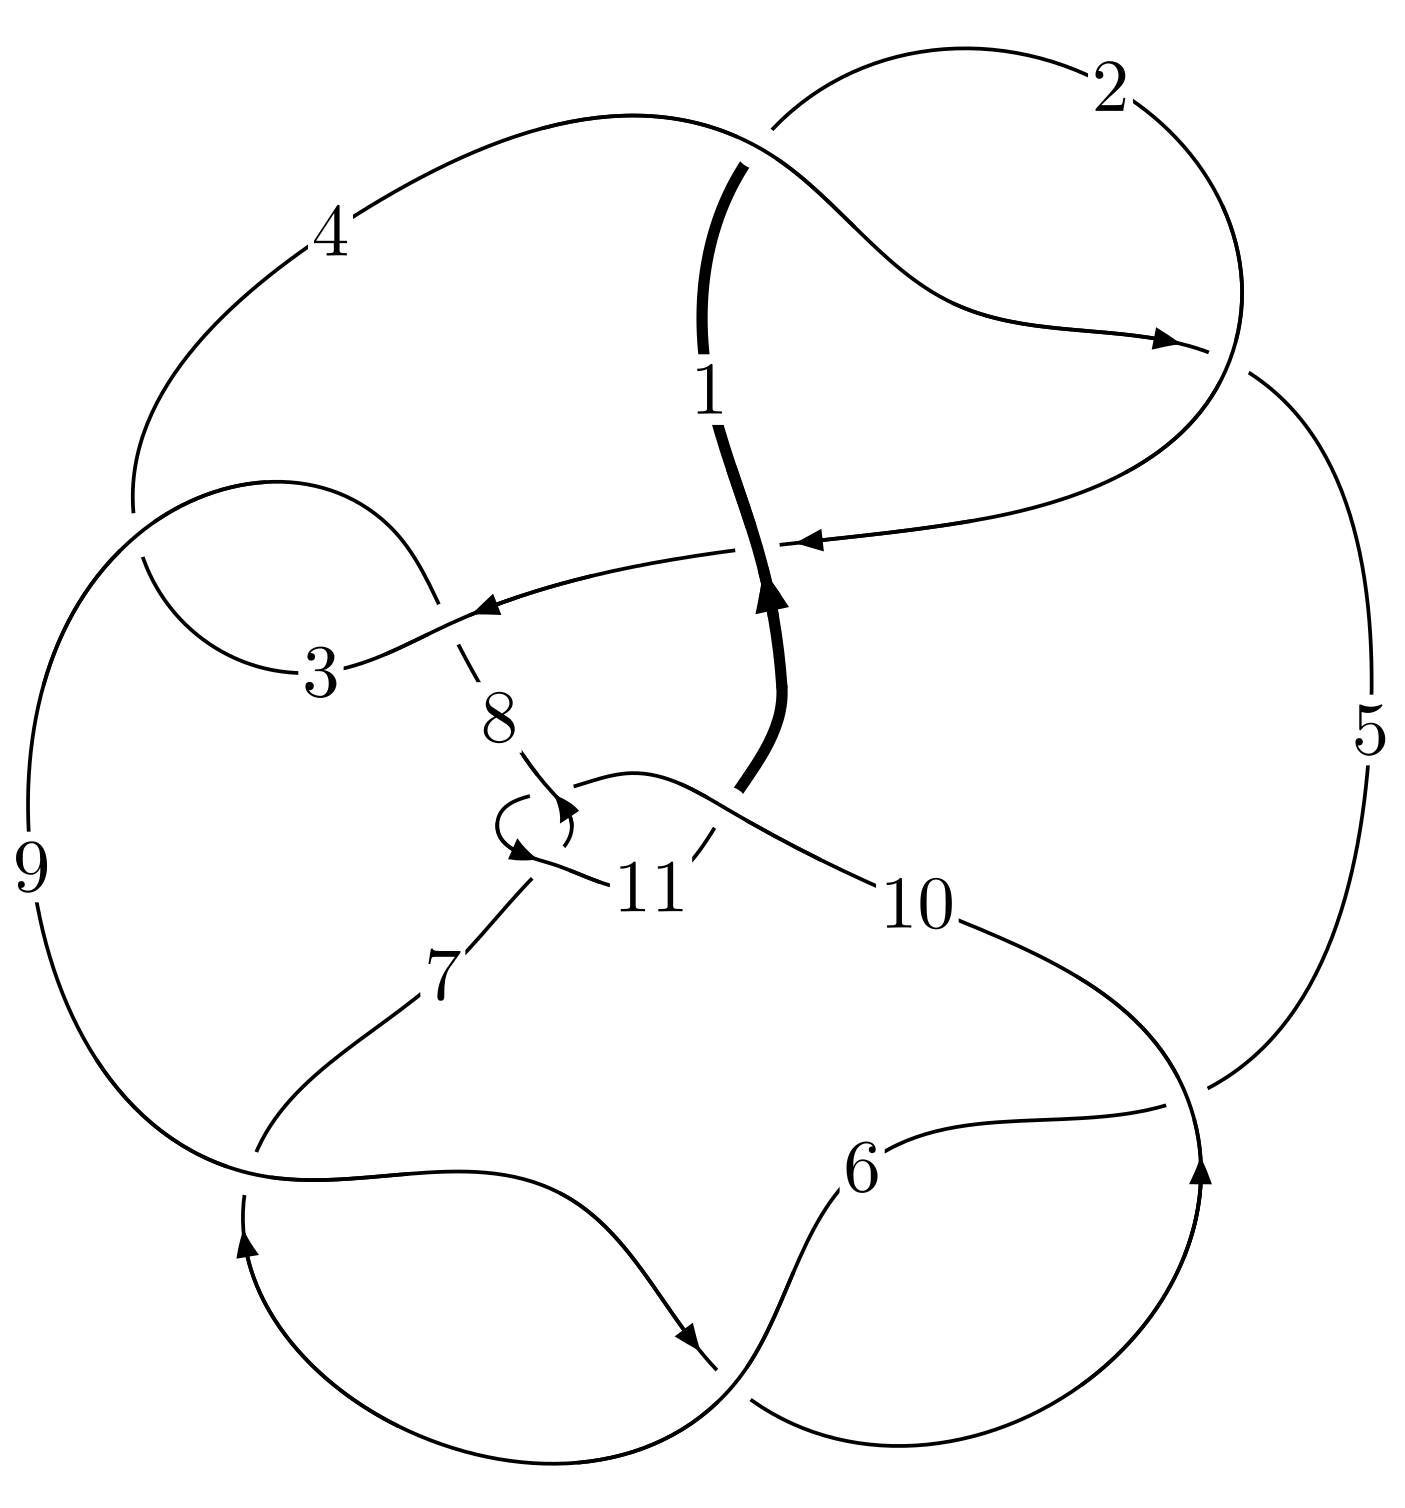
\includegraphics[width=112pt]{../../../GIT/diagram.site/Diagrams/png/682_11n_66.png}\\
\ \ \ A knot diagram\footnotemark}&
\allowdisplaybreaks
\textbf{Linearized knot diagam} \\
\cline{2-2}
 &
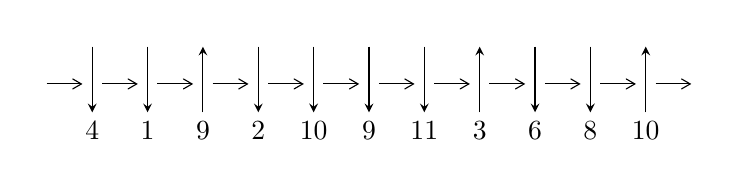
\begin{tikzpicture}[x=20pt, y=17pt]
	% nodes
	\node (C0) at (0, 0) {};
	\node (C1) at (1, 0) {};
	\node (C1U) at (1, +1) {};
	\node (C1D) at (1, -1) {4};

	\node (C2) at (2, 0) {};
	\node (C2U) at (2, +1) {};
	\node (C2D) at (2, -1) {1};

	\node (C3) at (3, 0) {};
	\node (C3U) at (3, +1) {};
	\node (C3D) at (3, -1) {9};

	\node (C4) at (4, 0) {};
	\node (C4U) at (4, +1) {};
	\node (C4D) at (4, -1) {2};

	\node (C5) at (5, 0) {};
	\node (C5U) at (5, +1) {};
	\node (C5D) at (5, -1) {10};

	\node (C6) at (6, 0) {};
	\node (C6U) at (6, +1) {};
	\node (C6D) at (6, -1) {9};

	\node (C7) at (7, 0) {};
	\node (C7U) at (7, +1) {};
	\node (C7D) at (7, -1) {11};

	\node (C8) at (8, 0) {};
	\node (C8U) at (8, +1) {};
	\node (C8D) at (8, -1) {3};

	\node (C9) at (9, 0) {};
	\node (C9U) at (9, +1) {};
	\node (C9D) at (9, -1) {6};

	\node (C10) at (10, 0) {};
	\node (C10U) at (10, +1) {};
	\node (C10D) at (10, -1) {8};

	\node (C11) at (11, 0) {};
	\node (C11U) at (11, +1) {};
	\node (C11D) at (11, -1) {10};
	\node (C12) at (12, 0) {};

	% arrows
	\draw[->,>={angle 60}]
	(C0) edge (C1) (C1) edge (C2) (C2) edge (C3) (C3) edge (C4) (C4) edge (C5) (C5) edge (C6) (C6) edge (C7) (C7) edge (C8) (C8) edge (C9) (C9) edge (C10) (C10) edge (C11) (C11) edge (C12) ;	\draw[->,>=stealth]
	(C1U) edge (C1D) (C2U) edge (C2D) (C3D) edge (C3U) (C4U) edge (C4D) (C5U) edge (C5D) (C6U) edge (C6D) (C7U) edge (C7D) (C8D) edge (C8U) (C9U) edge (C9D) (C10U) edge (C10D) (C11D) edge (C11U) ;
	\end{tikzpicture} \\
\hhline{~~} \\& 
\textbf{Solving Sequence} \\ \cline{2-2} 
 &
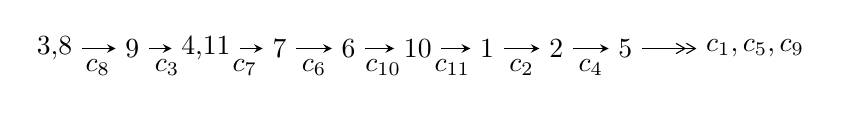
\begin{tikzpicture}[x=25pt, y=7pt]
	% node
	\node (A0) at (-1/8, 0) {3,8};
	\node (A1) at (1, 0) {9};
	\node (A2) at (33/16, 0) {4,11};
	\node (A3) at (25/8, 0) {7};
	\node (A4) at (33/8, 0) {6};
	\node (A5) at (41/8, 0) {10};
	\node (A6) at (49/8, 0) {1};
	\node (A7) at (57/8, 0) {2};
	\node (A8) at (65/8, 0) {5};
	\node (C1) at (1/2, -1) {$c_{8}$};
	\node (C2) at (3/2, -1) {$c_{3}$};
	\node (C3) at (21/8, -1) {$c_{7}$};
	\node (C4) at (29/8, -1) {$c_{6}$};
	\node (C5) at (37/8, -1) {$c_{10}$};
	\node (C6) at (45/8, -1) {$c_{11}$};
	\node (C7) at (53/8, -1) {$c_{2}$};
	\node (C8) at (61/8, -1) {$c_{4}$};
	\node (A9) at (10, 0) {$c_{1},c_{5},c_{9}$};

	% edge
	\draw[->,>=stealth]	
	(A0) edge (A1) (A1) edge (A2) (A2) edge (A3) (A3) edge (A4) (A4) edge (A5) (A5) edge (A6) (A6) edge (A7) (A7) edge (A8) ;
	\draw[->>,>={angle 60}]	
	(A8) edge (A9);
\end{tikzpicture} \\ 

\end{tabular} \\

\footnotetext{
The image of knot diagram is generated by the software ``\textbf{Draw programme}" developed by Andrew Bartholomew(\url{http://www.layer8.co.uk/maths/draw/index.htm\#Running-draw}), where we modified some parts for our purpose(\url{https://github.com/CATsTAILs/LinksPainter}).
}\phantom \\ \newline 
\centering \textbf{Ideals for irreducible components\footnotemark of $X_{\text{par}}$} 
 
\begin{align*}
I^u_{1}&=\langle 
4750254357724 u^{19}+14627504028936 u^{18}+\cdots+23633551708361 b-81147234294199,\\
\phantom{I^u_{1}}&\phantom{= \langle  }-74233627976373 u^{19}-270771524553115 u^{18}+\cdots+378136827333776 a+1442548033804746,\\
\phantom{I^u_{1}}&\phantom{= \langle  }u^{20}+3 u^{19}+\cdots-6 u+8\rangle \\
I^u_{2}&=\langle 
u^2 a+b+1,\;-2 u^{10} a-6 u^{11}+\cdots+a-2,\\
\phantom{I^u_{2}}&\phantom{= \langle  }u^{12}- u^{11}- u^{10}+2 u^9+3 u^8-4 u^7-2 u^6+4 u^5+2 u^4-3 u^3- u^2+1\rangle \\
I^u_{3}&=\langle 
- u^5+2 u^3+b- u,\;- u^4+2 u^3+3 u^2+a-3 u-2,\;u^6-3 u^4+2 u^2+1\rangle \\
\\
I^v_{1}&=\langle 
a,\;b-1,\;2 v+1\rangle \\
\end{align*}
\raggedright * 4 irreducible components of $\dim_{\mathbb{C}}=0$, with total 51 representations.\\
\footnotetext{All coefficients of polynomials are rational numbers. But the coefficients are sometimes approximated in decimal forms when there is not enough margin.}
\newpage
\renewcommand{\arraystretch}{1}
\centering \section*{I. $I^u_{1}= \langle 4.75\times10^{12} u^{19}+1.46\times10^{13} u^{18}+\cdots+2.36\times10^{13} b-8.11\times10^{13},\;-7.42\times10^{13} u^{19}-2.71\times10^{14} u^{18}+\cdots+3.78\times10^{14} a+1.44\times10^{15},\;u^{20}+3 u^{19}+\cdots-6 u+8 \rangle$}
\flushleft \textbf{(i) Arc colorings}\\
\begin{tabular}{m{7pt} m{180pt} m{7pt} m{180pt} }
\flushright $a_{3}=$&$\begin{pmatrix}0\\u\end{pmatrix}$ \\
\flushright $a_{8}=$&$\begin{pmatrix}1\\0\end{pmatrix}$ \\
\flushright $a_{9}=$&$\begin{pmatrix}1\\- u^2\end{pmatrix}$ \\
\flushright $a_{4}=$&$\begin{pmatrix}u\\- u^3+u\end{pmatrix}$ \\
\flushright $a_{11}=$&$\begin{pmatrix}0.196314 u^{19}+0.716068 u^{18}+\cdots-3.73611 u-3.81488\\-0.200996 u^{19}-0.618930 u^{18}+\cdots+3.09511 u+3.43356\end{pmatrix}$ \\
\flushright $a_{7}=$&$\begin{pmatrix}-0.00468201 u^{19}+0.0971380 u^{18}+\cdots-0.640997 u-0.381323\\0.238201 u^{19}+0.712561 u^{18}+\cdots-3.79968 u-2.54409\end{pmatrix}$ \\
\flushright $a_{6}=$&$\begin{pmatrix}0.196314 u^{19}+0.716068 u^{18}+\cdots-3.73611 u-3.81488\\0.107586 u^{19}+0.364861 u^{18}+\cdots-2.28735 u-2.41656\end{pmatrix}$ \\
\flushright $a_{10}=$&$\begin{pmatrix}-0.00468201 u^{19}+0.0971380 u^{18}+\cdots-0.640997 u-0.381323\\-0.200996 u^{19}-0.618930 u^{18}+\cdots+3.09511 u+3.43356\end{pmatrix}$ \\
\flushright $a_{1}=$&$\begin{pmatrix}-0.0380706 u^{19}+0.0221177 u^{18}+\cdots-0.0686952 u-0.889509\\-0.467904 u^{19}-1.50365 u^{18}+\cdots+8.10809 u+6.85079\end{pmatrix}$ \\
\flushright $a_{2}=$&$\begin{pmatrix}0.0279992 u^{19}+0.365360 u^{18}+\cdots-2.48168 u-2.62009\\-0.344443 u^{19}-1.03168 u^{18}+\cdots+5.35346 u+6.28047\end{pmatrix}$ \\
\flushright $a_{5}=$&$\begin{pmatrix}-0.429833 u^{19}-1.52577 u^{18}+\cdots+8.17678 u+7.74030\\-0.345787 u^{19}-1.07742 u^{18}+\cdots+6.08703 u+4.96065\end{pmatrix}$\\ \flushright $a_{5}=$&$\begin{pmatrix}-0.429833 u^{19}-1.52577 u^{18}+\cdots+8.17678 u+7.74030\\-0.345787 u^{19}-1.07742 u^{18}+\cdots+6.08703 u+4.96065\end{pmatrix}$\\&\end{tabular}
\flushleft \textbf{(ii) Obstruction class $= -1$}\\~\\
\flushleft \textbf{(iii) Cusp Shapes $= -\frac{29166765795697}{27009773380984} u^{19}-\frac{107025259759479}{27009773380984} u^{18}+\cdots+\frac{889027178406181}{27009773380984} u+\frac{218402675148733}{13504886690492}$}\\~\\
\newpage\renewcommand{\arraystretch}{1}
\flushleft \textbf{(iv) u-Polynomials at the component}\newline \\
\begin{tabular}{m{50pt}|m{274pt}}
Crossings & \hspace{64pt}u-Polynomials at each crossing \\
\hline $$\begin{aligned}c_{1},c_{4}\end{aligned}$$&$\begin{aligned}
&u^{20}-2 u^{19}+\cdots-3 u-4
\end{aligned}$\\
\hline $$\begin{aligned}c_{2}\end{aligned}$$&$\begin{aligned}
&u^{20}+10 u^{19}+\cdots+65 u+16
\end{aligned}$\\
\hline $$\begin{aligned}c_{3},c_{8}\end{aligned}$$&$\begin{aligned}
&u^{20}-3 u^{19}+\cdots+6 u+8
\end{aligned}$\\
\hline $$\begin{aligned}c_{5},c_{6},c_{7}\\c_{9},c_{10}\end{aligned}$$&$\begin{aligned}
&u^{20}+u^{19}+\cdots+u^2-1
\end{aligned}$\\
\hline $$\begin{aligned}c_{11}\end{aligned}$$&$\begin{aligned}
&u^{20}-5 u^{19}+\cdots+2 u+1
\end{aligned}$\\
\hline
\end{tabular}\\~\\
\newpage\renewcommand{\arraystretch}{1}
\flushleft \textbf{(v) Riley Polynomials at the component}\newline \\
\begin{tabular}{m{50pt}|m{274pt}}
Crossings & \hspace{64pt}Riley Polynomials at each crossing \\
\hline $$\begin{aligned}c_{1},c_{4}\end{aligned}$$&$\begin{aligned}
&y^{20}-10 y^{19}+\cdots-65 y+16
\end{aligned}$\\
\hline $$\begin{aligned}c_{2}\end{aligned}$$&$\begin{aligned}
&y^{20}+2 y^{19}+\cdots+3935 y+256
\end{aligned}$\\
\hline $$\begin{aligned}c_{3},c_{8}\end{aligned}$$&$\begin{aligned}
&y^{20}-9 y^{19}+\cdots-372 y+64
\end{aligned}$\\
\hline $$\begin{aligned}c_{5},c_{6},c_{7}\\c_{9},c_{10}\end{aligned}$$&$\begin{aligned}
&y^{20}+5 y^{19}+\cdots-2 y+1
\end{aligned}$\\
\hline $$\begin{aligned}c_{11}\end{aligned}$$&$\begin{aligned}
&y^{20}+21 y^{19}+\cdots-26 y+1
\end{aligned}$\\
\hline
\end{tabular}\\~\\
\newpage\flushleft \textbf{(vi) Complex Volumes and Cusp Shapes}
$$\begin{array}{c|c|c}  
\text{Solutions to }I^u_{1}& \I (\text{vol} + \sqrt{-1}CS) & \text{Cusp shape}\\
 \hline 
\begin{aligned}
u &= -0.673179 + 0.716265 I \\
a &= -0.148792 + 0.308519 I \\
b &= \phantom{-}1.076780 - 0.752726 I\end{aligned}
 & -5.39578 - 0.84915 I & -7.95749 + 2.97696 I \\ \hline\begin{aligned}
u &= -0.673179 - 0.716265 I \\
a &= -0.148792 - 0.308519 I \\
b &= \phantom{-}1.076780 + 0.752726 I\end{aligned}
 & -5.39578 + 0.84915 I & -7.95749 - 2.97696 I \\ \hline\begin{aligned}
u &= \phantom{-}0.457611 + 1.029390 I \\
a &= -0.041132 - 0.464695 I \\
b &= \phantom{-}0.689086 + 0.818580 I\end{aligned}
 & -1.13732 - 2.28200 I & -3.79248 + 2.52259 I \\ \hline\begin{aligned}
u &= \phantom{-}0.457611 - 1.029390 I \\
a &= -0.041132 + 0.464695 I \\
b &= \phantom{-}0.689086 - 0.818580 I\end{aligned}
 & -1.13732 + 2.28200 I & -3.79248 - 2.52259 I \\ \hline\begin{aligned}
u &= -1.057230 + 0.616811 I \\
a &= -0.48847 + 1.97668 I \\
b &= -0.754597 - 0.948291 I\end{aligned}
 & -4.17399 - 4.33843 I & -5.43818 + 4.87758 I \\ \hline\begin{aligned}
u &= -1.057230 - 0.616811 I \\
a &= -0.48847 - 1.97668 I \\
b &= -0.754597 + 0.948291 I\end{aligned}
 & -4.17399 + 4.33843 I & -5.43818 - 4.87758 I \\ \hline\begin{aligned}
u &= -0.114291 + 0.713759 I \\
a &= \phantom{-}0.381764 - 0.379380 I \\
b &= \phantom{-}0.345961 + 0.369550 I\end{aligned}
 & -0.507859 - 1.098400 I & -5.66835 + 6.51867 I \\ \hline\begin{aligned}
u &= -0.114291 - 0.713759 I \\
a &= \phantom{-}0.381764 + 0.379380 I \\
b &= \phantom{-}0.345961 - 0.369550 I\end{aligned}
 & -0.507859 + 1.098400 I & -5.66835 - 6.51867 I \\ \hline\begin{aligned}
u &= -0.686172 + 1.114670 I \\
a &= -0.149939 + 0.505520 I \\
b &= \phantom{-}0.738092 - 1.033620 I\end{aligned}
 & -3.56378 + 7.37420 I & -5.16607 - 5.93843 I \\ \hline\begin{aligned}
u &= -0.686172 - 1.114670 I \\
a &= -0.149939 - 0.505520 I \\
b &= \phantom{-}0.738092 + 1.033620 I\end{aligned}
 & -3.56378 - 7.37420 I & -5.16607 + 5.93843 I\\
 \hline 
 \end{array}$$\newpage$$\begin{array}{c|c|c}  
\text{Solutions to }I^u_{1}& \I (\text{vol} + \sqrt{-1}CS) & \text{Cusp shape}\\
 \hline 
\begin{aligned}
u &= \phantom{-}1.20041 + 0.74865 I \\
a &= -0.52942 - 1.65229 I \\
b &= -0.681127 + 1.119630 I\end{aligned}
 & \phantom{-}1.09912 + 8.73296 I & -0.91420 - 6.11492 I \\ \hline\begin{aligned}
u &= \phantom{-}1.20041 - 0.74865 I \\
a &= -0.52942 + 1.65229 I \\
b &= -0.681127 - 1.119630 I\end{aligned}
 & \phantom{-}1.09912 - 8.73296 I & -0.91420 + 6.11492 I \\ \hline\begin{aligned}
u &= -1.15925 + 0.84659 I \\
a &= -0.67085 + 1.58475 I \\
b &= -0.74872 - 1.20984 I\end{aligned}
 & -2.0375 - 14.4341 I & -3.68264 + 8.80511 I \\ \hline\begin{aligned}
u &= -1.15925 - 0.84659 I \\
a &= -0.67085 - 1.58475 I \\
b &= -0.74872 + 1.20984 I\end{aligned}
 & -2.0375 + 14.4341 I & -3.68264 - 8.80511 I \\ \hline\begin{aligned}
u &= -1.44359 + 0.25308 I \\
a &= \phantom{-}0.295484 - 1.320210 I \\
b &= -0.242677 + 0.771774 I\end{aligned}
 & \phantom{-}5.28190 - 1.85243 I & -3.45872 - 2.75624 I \\ \hline\begin{aligned}
u &= -1.44359 - 0.25308 I \\
a &= \phantom{-}0.295484 + 1.320210 I \\
b &= -0.242677 - 0.771774 I\end{aligned}
 & \phantom{-}5.28190 + 1.85243 I & -3.45872 + 2.75624 I \\ \hline\begin{aligned}
u &= \phantom{-}0.527412\phantom{ +0.000000I} \\
a &= \phantom{-}2.13544\phantom{ +0.000000I} \\
b &= -0.362131\phantom{ +0.000000I}\end{aligned}
 & -2.14785\phantom{ +0.000000I} & -2.01910\phantom{ +0.000000I} \\ \hline\begin{aligned}
u &= \phantom{-}1.47329 + 0.10154 I \\
a &= \phantom{-}0.14365 - 1.48101 I \\
b &= -0.346734 + 0.845969 I\end{aligned}
 & \phantom{-}5.55307 + 4.39884 I & -1.65086 - 8.29154 I \\ \hline\begin{aligned}
u &= \phantom{-}1.47329 - 0.10154 I \\
a &= \phantom{-}0.14365 + 1.48101 I \\
b &= -0.346734 - 0.845969 I\end{aligned}
 & \phantom{-}5.55307 - 4.39884 I & -1.65086 + 8.29154 I \\ \hline\begin{aligned}
u &= \phantom{-}0.477398\phantom{ +0.000000I} \\
a &= -0.0950270\phantom{ +0.000000I} \\
b &= \phantom{-}1.21001\phantom{ +0.000000I}\end{aligned}
 & -2.89220\phantom{ +0.000000I} & \phantom{-}7.72710\phantom{ +0.000000I}\\
 \hline 
 \end{array}$$\newpage\newpage\renewcommand{\arraystretch}{1}
\centering \section*{II. $I^u_{2}= \langle u^2 a+b+1,\;-2 u^{10} a-6 u^{11}+\cdots+a-2,\;u^{12}- u^{11}+\cdots- u^2+1 \rangle$}
\flushleft \textbf{(i) Arc colorings}\\
\begin{tabular}{m{7pt} m{180pt} m{7pt} m{180pt} }
\flushright $a_{3}=$&$\begin{pmatrix}0\\u\end{pmatrix}$ \\
\flushright $a_{8}=$&$\begin{pmatrix}1\\0\end{pmatrix}$ \\
\flushright $a_{9}=$&$\begin{pmatrix}1\\- u^2\end{pmatrix}$ \\
\flushright $a_{4}=$&$\begin{pmatrix}u\\- u^3+u\end{pmatrix}$ \\
\flushright $a_{11}=$&$\begin{pmatrix}a\\- u^2 a-1\end{pmatrix}$ \\
\flushright $a_{7}=$&$\begin{pmatrix}2 u^{10}-2 u^9-2 u^8+4 u^7+6 u^6-8 u^5-4 u^4+u^2 a+8 u^3+3 u^2- a-6 u\\- u^4 a+u^4- u^2+1\end{pmatrix}$ \\
\flushright $a_{6}=$&$\begin{pmatrix}2 u^{10}-2 u^9-2 u^8+4 u^7+6 u^6-8 u^5-4 u^4+8 u^3+4 u^2- a-6 u-1\\1\end{pmatrix}$ \\
\flushright $a_{10}=$&$\begin{pmatrix}- u^2 a+a-1\\- u^2 a-1\end{pmatrix}$ \\
\flushright $a_{1}=$&$\begin{pmatrix}u^6- u^4+2 u^2-1\\u^6+u^2\end{pmatrix}$ \\
\flushright $a_{2}=$&$\begin{pmatrix}- u^{10}+u^8-2 u^6+u^4+u^2-1\\u^{11}- u^{10}-2 u^9+u^8+4 u^7-2 u^6-4 u^5+u^4+3 u^3+u^2-1\end{pmatrix}$ \\
\flushright $a_{5}=$&$\begin{pmatrix}u^4- u^2+1\\u^4\end{pmatrix}$\\ \flushright $a_{5}=$&$\begin{pmatrix}u^4- u^2+1\\u^4\end{pmatrix}$\\&\end{tabular}
\flushleft \textbf{(ii) Obstruction class $= -1$}\\~\\
\flushleft \textbf{(iii) Cusp Shapes $= -4 u^{11}+8 u^9-4 u^8-16 u^7+4 u^6+20 u^5-8 u^4-12 u^3+4 u^2+8 u-2$}\\~\\
\newpage\renewcommand{\arraystretch}{1}
\flushleft \textbf{(iv) u-Polynomials at the component}\newline \\
\begin{tabular}{m{50pt}|m{274pt}}
Crossings & \hspace{64pt}u-Polynomials at each crossing \\
\hline $$\begin{aligned}c_{1},c_{4}\end{aligned}$$&$\begin{aligned}
&(u^{12}- u^{11}+\cdots-2 u+1)^{2}
\end{aligned}$\\
\hline $$\begin{aligned}c_{2}\end{aligned}$$&$\begin{aligned}
&(u^{12}+7 u^{11}+\cdots+2 u+1)^{2}
\end{aligned}$\\
\hline $$\begin{aligned}c_{3},c_{8}\end{aligned}$$&$\begin{aligned}
&(u^{12}+u^{11}- u^{10}-2 u^9+3 u^8+4 u^7-2 u^6-4 u^5+2 u^4+3 u^3- u^2+1)^2
\end{aligned}$\\
\hline $$\begin{aligned}c_{5},c_{6},c_{7}\\c_{9},c_{10}\end{aligned}$$&$\begin{aligned}
&u^{24}-3 u^{23}+\cdots-52 u+17
\end{aligned}$\\
\hline $$\begin{aligned}c_{11}\end{aligned}$$&$\begin{aligned}
&u^{24}-11 u^{23}+\cdots-1784 u+289
\end{aligned}$\\
\hline
\end{tabular}\\~\\
\newpage\renewcommand{\arraystretch}{1}
\flushleft \textbf{(v) Riley Polynomials at the component}\newline \\
\begin{tabular}{m{50pt}|m{274pt}}
Crossings & \hspace{64pt}Riley Polynomials at each crossing \\
\hline $$\begin{aligned}c_{1},c_{4}\end{aligned}$$&$\begin{aligned}
&(y^{12}-7 y^{11}+\cdots-2 y+1)^{2}
\end{aligned}$\\
\hline $$\begin{aligned}c_{2}\end{aligned}$$&$\begin{aligned}
&(y^{12}-3 y^{11}+\cdots+6 y+1)^{2}
\end{aligned}$\\
\hline $$\begin{aligned}c_{3},c_{8}\end{aligned}$$&$\begin{aligned}
&(y^{12}-3 y^{11}+\cdots-2 y+1)^{2}
\end{aligned}$\\
\hline $$\begin{aligned}c_{5},c_{6},c_{7}\\c_{9},c_{10}\end{aligned}$$&$\begin{aligned}
&y^{24}+11 y^{23}+\cdots+1784 y+289
\end{aligned}$\\
\hline $$\begin{aligned}c_{11}\end{aligned}$$&$\begin{aligned}
&y^{24}+3 y^{23}+\cdots+158184 y+83521
\end{aligned}$\\
\hline
\end{tabular}\\~\\
\newpage\flushleft \textbf{(vi) Complex Volumes and Cusp Shapes}
$$\begin{array}{c|c|c}  
\text{Solutions to }I^u_{2}& \I (\text{vol} + \sqrt{-1}CS) & \text{Cusp shape}\\
 \hline 
\begin{aligned}
u &= -0.915752 + 0.387588 I \\
a &= -0.719269 + 0.265989 I \\
b &= -0.693689 - 0.693688 I\end{aligned}
 & \phantom{-}3.36661 - 4.24921 I & -1.82351 + 6.98310 I \\ \hline\begin{aligned}
u &= -0.915752 + 0.387588 I \\
a &= \phantom{-}0.31123 - 1.71799 I \\
b &= \phantom{-}0.005311 + 1.403560 I\end{aligned}
 & \phantom{-}3.36661 - 4.24921 I & -1.82351 + 6.98310 I \\ \hline\begin{aligned}
u &= -0.915752 - 0.387588 I \\
a &= -0.719269 - 0.265989 I \\
b &= -0.693689 + 0.693688 I\end{aligned}
 & \phantom{-}3.36661 + 4.24921 I & -1.82351 - 6.98310 I \\ \hline\begin{aligned}
u &= -0.915752 - 0.387588 I \\
a &= \phantom{-}0.31123 + 1.71799 I \\
b &= \phantom{-}0.005311 - 1.403560 I\end{aligned}
 & \phantom{-}3.36661 + 4.24921 I & -1.82351 - 6.98310 I \\ \hline\begin{aligned}
u &= \phantom{-}0.825437 + 0.157146 I \\
a &= -1.25892 - 1.03181 I \\
b &= -0.441009 + 1.004140 I\end{aligned}
 & \phantom{-}4.72717 + 0.35310 I & \phantom{-}2.66692 - 0.62981 I \\ \hline\begin{aligned}
u &= \phantom{-}0.825437 + 0.157146 I \\
a &= -0.37562 + 2.07265 I \\
b &= -0.215643 - 1.263560 I\end{aligned}
 & \phantom{-}4.72717 + 0.35310 I & \phantom{-}2.66692 - 0.62981 I \\ \hline\begin{aligned}
u &= \phantom{-}0.825437 - 0.157146 I \\
a &= -1.25892 + 1.03181 I \\
b &= -0.441009 - 1.004140 I\end{aligned}
 & \phantom{-}4.72717 - 0.35310 I & \phantom{-}2.66692 + 0.62981 I \\ \hline\begin{aligned}
u &= \phantom{-}0.825437 - 0.157146 I \\
a &= -0.37562 - 2.07265 I \\
b &= -0.215643 + 1.263560 I\end{aligned}
 & \phantom{-}4.72717 - 0.35310 I & \phantom{-}2.66692 + 0.62981 I \\ \hline\begin{aligned}
u &= -0.895445 + 0.803537 I \\
a &= \phantom{-}0.520071 - 1.227910 I \\
b &= \phantom{-}0.685814 + 0.940144 I\end{aligned}
 & -0.75031 - 3.01307 I & -3.36825 + 2.63251 I \\ \hline\begin{aligned}
u &= -0.895445 + 0.803537 I \\
a &= \phantom{-}0.330877 - 0.145723 I \\
b &= -0.841964 + 0.498902 I\end{aligned}
 & -0.75031 - 3.01307 I & -3.36825 + 2.63251 I\\
 \hline 
 \end{array}$$\newpage$$\begin{array}{c|c|c}  
\text{Solutions to }I^u_{2}& \I (\text{vol} + \sqrt{-1}CS) & \text{Cusp shape}\\
 \hline 
\begin{aligned}
u &= -0.895445 - 0.803537 I \\
a &= \phantom{-}0.520071 + 1.227910 I \\
b &= \phantom{-}0.685814 - 0.940144 I\end{aligned}
 & -0.75031 + 3.01307 I & -3.36825 - 2.63251 I \\ \hline\begin{aligned}
u &= -0.895445 - 0.803537 I \\
a &= \phantom{-}0.330877 + 0.145723 I \\
b &= -0.841964 - 0.498902 I\end{aligned}
 & -0.75031 + 3.01307 I & -3.36825 - 2.63251 I \\ \hline\begin{aligned}
u &= \phantom{-}0.849698 + 0.874392 I \\
a &= \phantom{-}0.495565 + 1.219030 I \\
b &= \phantom{-}0.832505 - 0.684481 I\end{aligned}
 & -4.62532 - 1.48234 I & -7.15258 + 0.67542 I \\ \hline\begin{aligned}
u &= \phantom{-}0.849698 + 0.874392 I \\
a &= \phantom{-}0.542966 + 0.125815 I \\
b &= -0.789930 - 0.801459 I\end{aligned}
 & -4.62532 - 1.48234 I & -7.15258 + 0.67542 I \\ \hline\begin{aligned}
u &= \phantom{-}0.849698 - 0.874392 I \\
a &= \phantom{-}0.495565 - 1.219030 I \\
b &= \phantom{-}0.832505 + 0.684481 I\end{aligned}
 & -4.62532 + 1.48234 I & -7.15258 - 0.67542 I \\ \hline\begin{aligned}
u &= \phantom{-}0.849698 - 0.874392 I \\
a &= \phantom{-}0.542966 - 0.125815 I \\
b &= -0.789930 + 0.801459 I\end{aligned}
 & -4.62532 + 1.48234 I & -7.15258 - 0.67542 I \\ \hline\begin{aligned}
u &= \phantom{-}0.962887 + 0.828850 I \\
a &= \phantom{-}0.498094 + 1.238190 I \\
b &= \phantom{-}0.856755 - 1.092410 I\end{aligned}
 & -4.26829 + 7.80134 I & -6.36611 - 5.63981 I \\ \hline\begin{aligned}
u &= \phantom{-}0.962887 + 0.828850 I \\
a &= \phantom{-}0.317556 - 0.012937 I \\
b &= -1.096910 - 0.503770 I\end{aligned}
 & -4.26829 + 7.80134 I & -6.36611 - 5.63981 I \\ \hline\begin{aligned}
u &= \phantom{-}0.962887 - 0.828850 I \\
a &= \phantom{-}0.498094 - 1.238190 I \\
b &= \phantom{-}0.856755 + 1.092410 I\end{aligned}
 & -4.26829 - 7.80134 I & -6.36611 + 5.63981 I \\ \hline\begin{aligned}
u &= \phantom{-}0.962887 - 0.828850 I \\
a &= \phantom{-}0.317556 + 0.012937 I \\
b &= -1.096910 + 0.503770 I\end{aligned}
 & -4.26829 - 7.80134 I & -6.36611 + 5.63981 I\\
 \hline 
 \end{array}$$\newpage$$\begin{array}{c|c|c}  
\text{Solutions to }I^u_{2}& \I (\text{vol} + \sqrt{-1}CS) & \text{Cusp shape}\\
 \hline 
\begin{aligned}
u &= -0.326826 + 0.552791 I \\
a &= -0.32038 - 3.37299 I \\
b &= \phantom{-}0.155092 - 0.786191 I\end{aligned}
 & \phantom{-}1.55013 + 0.71593 I & -7.95647 - 0.64874 I \\ \hline\begin{aligned}
u &= -0.326826 + 0.552791 I \\
a &= \phantom{-}3.65784 - 0.87628 I \\
b &= \phantom{-}0.043670 + 1.147520 I\end{aligned}
 & \phantom{-}1.55013 + 0.71593 I & -7.95647 - 0.64874 I \\ \hline\begin{aligned}
u &= -0.326826 - 0.552791 I \\
a &= -0.32038 + 3.37299 I \\
b &= \phantom{-}0.155092 + 0.786191 I\end{aligned}
 & \phantom{-}1.55013 - 0.71593 I & -7.95647 + 0.64874 I \\ \hline\begin{aligned}
u &= -0.326826 - 0.552791 I \\
a &= \phantom{-}3.65784 + 0.87628 I \\
b &= \phantom{-}0.043670 - 1.147520 I\end{aligned}
 & \phantom{-}1.55013 - 0.71593 I & -7.95647 + 0.64874 I\\
 \hline 
 \end{array}$$\newpage\newpage\renewcommand{\arraystretch}{1}
\centering \section*{III. $I^u_{3}= \langle - u^5+2 u^3+b- u,\;- u^4+2 u^3+3 u^2+a-3 u-2,\;u^6-3 u^4+2 u^2+1 \rangle$}
\flushleft \textbf{(i) Arc colorings}\\
\begin{tabular}{m{7pt} m{180pt} m{7pt} m{180pt} }
\flushright $a_{3}=$&$\begin{pmatrix}0\\u\end{pmatrix}$ \\
\flushright $a_{8}=$&$\begin{pmatrix}1\\0\end{pmatrix}$ \\
\flushright $a_{9}=$&$\begin{pmatrix}1\\- u^2\end{pmatrix}$ \\
\flushright $a_{4}=$&$\begin{pmatrix}u\\- u^3+u\end{pmatrix}$ \\
\flushright $a_{11}=$&$\begin{pmatrix}u^4-2 u^3-3 u^2+3 u+2\\u^5-2 u^3+u\end{pmatrix}$ \\
\flushright $a_{7}=$&$\begin{pmatrix}- u^5+u^4+4 u^3-3 u^2-4 u+2\\1\end{pmatrix}$ \\
\flushright $a_{6}=$&$\begin{pmatrix}u^4+2 u^3-3 u^2-3 u+2\\- u^5+u^3+u+1\end{pmatrix}$ \\
\flushright $a_{10}=$&$\begin{pmatrix}u^5+u^4-4 u^3-3 u^2+4 u+2\\u^5-2 u^3+u\end{pmatrix}$ \\
\flushright $a_{1}=$&$\begin{pmatrix}- u^5+2 u^3- u\\0\end{pmatrix}$ \\
\flushright $a_{2}=$&$\begin{pmatrix}- u\\u\end{pmatrix}$ \\
\flushright $a_{5}=$&$\begin{pmatrix}u^5-2 u^3+u\\- u^5+u^3+u\end{pmatrix}$\\ \flushright $a_{5}=$&$\begin{pmatrix}u^5-2 u^3+u\\- u^5+u^3+u\end{pmatrix}$\\&\end{tabular}
\flushleft \textbf{(ii) Obstruction class $= 1$}\\~\\
\flushleft \textbf{(iii) Cusp Shapes $= -4 u^4+8 u^2$}\\~\\
\newpage\renewcommand{\arraystretch}{1}
\flushleft \textbf{(iv) u-Polynomials at the component}\newline \\
\begin{tabular}{m{50pt}|m{274pt}}
Crossings & \hspace{64pt}u-Polynomials at each crossing \\
\hline $$\begin{aligned}c_{1}\end{aligned}$$&$\begin{aligned}
&(u^3+u^2-1)^2
\end{aligned}$\\
\hline $$\begin{aligned}c_{2}\end{aligned}$$&$\begin{aligned}
&(u^3+u^2+2 u+1)^2
\end{aligned}$\\
\hline $$\begin{aligned}c_{3},c_{8}\end{aligned}$$&$\begin{aligned}
&u^6-3 u^4+2 u^2+1
\end{aligned}$\\
\hline $$\begin{aligned}c_{4}\end{aligned}$$&$\begin{aligned}
&(u^3- u^2+1)^2
\end{aligned}$\\
\hline $$\begin{aligned}c_{5},c_{6},c_{7}\\c_{9},c_{10}\end{aligned}$$&$\begin{aligned}
&(u^2+1)^3
\end{aligned}$\\
\hline $$\begin{aligned}c_{11}\end{aligned}$$&$\begin{aligned}
&(u-1)^6
\end{aligned}$\\
\hline
\end{tabular}\\~\\
\newpage\renewcommand{\arraystretch}{1}
\flushleft \textbf{(v) Riley Polynomials at the component}\newline \\
\begin{tabular}{m{50pt}|m{274pt}}
Crossings & \hspace{64pt}Riley Polynomials at each crossing \\
\hline $$\begin{aligned}c_{1},c_{4}\end{aligned}$$&$\begin{aligned}
&(y^3- y^2+2 y-1)^2
\end{aligned}$\\
\hline $$\begin{aligned}c_{2}\end{aligned}$$&$\begin{aligned}
&(y^3+3 y^2+2 y-1)^2
\end{aligned}$\\
\hline $$\begin{aligned}c_{3},c_{8}\end{aligned}$$&$\begin{aligned}
&(y^3-3 y^2+2 y+1)^2
\end{aligned}$\\
\hline $$\begin{aligned}c_{5},c_{6},c_{7}\\c_{9},c_{10}\end{aligned}$$&$\begin{aligned}
&(y+1)^6
\end{aligned}$\\
\hline $$\begin{aligned}c_{11}\end{aligned}$$&$\begin{aligned}
&(y-1)^6
\end{aligned}$\\
\hline
\end{tabular}\\~\\
\newpage\flushleft \textbf{(vi) Complex Volumes and Cusp Shapes}
$$\begin{array}{c|c|c}  
\text{Solutions to }I^u_{3}& \I (\text{vol} + \sqrt{-1}CS) & \text{Cusp shape}\\
 \hline 
\begin{aligned}
u &= \phantom{-}1.307140 + 0.215080 I \\
a &= -0.72238 - 1.35722 I \\
b &= \phantom{-0.000000 -}1.000000 I\end{aligned}
 & \phantom{-}6.31400 + 2.82812 I & \phantom{-}3.50976 - 2.97945 I \\ \hline\begin{aligned}
u &= \phantom{-}1.307140 - 0.215080 I \\
a &= -0.72238 + 1.35722 I \\
b &= \phantom{-0.000000 } -1.000000 I\end{aligned}
 & \phantom{-}6.31400 - 2.82812 I & \phantom{-}3.50976 + 2.97945 I \\ \hline\begin{aligned}
u &= -1.307140 + 0.215080 I \\
a &= -0.35722 - 1.72238 I \\
b &= \phantom{-0.000000 -}1.000000 I\end{aligned}
 & \phantom{-}6.31400 - 2.82812 I & \phantom{-}3.50976 + 2.97945 I \\ \hline\begin{aligned}
u &= -1.307140 - 0.215080 I \\
a &= -0.35722 + 1.72238 I \\
b &= \phantom{-0.000000 } -1.000000 I\end{aligned}
 & \phantom{-}6.31400 + 2.82812 I & \phantom{-}3.50976 - 2.97945 I \\ \hline\begin{aligned}
u &= \phantom{-0.000000 -}0.569840 I \\
a &= \phantom{-}3.07960 + 2.07960 I \\
b &= \phantom{-0.000000 -}1.000000 I\end{aligned}
 & \phantom{-}2.17641\phantom{ +0.000000I} & -3.01950\phantom{ +0.000000I} \\ \hline\begin{aligned}
u &= \phantom{-0.000000 } -0.569840 I \\
a &= \phantom{-}3.07960 - 2.07960 I \\
b &= \phantom{-0.000000 } -1.000000 I\end{aligned}
 & \phantom{-}2.17641\phantom{ +0.000000I} & -3.01950\phantom{ +0.000000I}\\
 \hline 
 \end{array}$$\newpage\newpage\renewcommand{\arraystretch}{1}
\centering \section*{IV. $I^v_{1}= \langle a,\;b-1,\;2 v+1 \rangle$}
\flushleft \textbf{(i) Arc colorings}\\
\begin{tabular}{m{7pt} m{180pt} m{7pt} m{180pt} }
\flushright $a_{3}=$&$\begin{pmatrix}-0.5\\0\end{pmatrix}$ \\
\flushright $a_{8}=$&$\begin{pmatrix}1\\0\end{pmatrix}$ \\
\flushright $a_{9}=$&$\begin{pmatrix}1\\0\end{pmatrix}$ \\
\flushright $a_{4}=$&$\begin{pmatrix}-0.5\\0\end{pmatrix}$ \\
\flushright $a_{11}=$&$\begin{pmatrix}0\\1\end{pmatrix}$ \\
\flushright $a_{7}=$&$\begin{pmatrix}1\\-1\end{pmatrix}$ \\
\flushright $a_{6}=$&$\begin{pmatrix}0\\-1\end{pmatrix}$ \\
\flushright $a_{10}=$&$\begin{pmatrix}1\\1\end{pmatrix}$ \\
\flushright $a_{1}=$&$\begin{pmatrix}1\\2\end{pmatrix}$ \\
\flushright $a_{2}=$&$\begin{pmatrix}0.5\\2\end{pmatrix}$ \\
\flushright $a_{5}=$&$\begin{pmatrix}-1\\-2\end{pmatrix}$\\ \flushright $a_{5}=$&$\begin{pmatrix}-1\\-2\end{pmatrix}$\\&\end{tabular}
\flushleft \textbf{(ii) Obstruction class $= 1$}\\~\\
\flushleft \textbf{(iii) Cusp Shapes $= -14.25$}\\~\\
\newpage\renewcommand{\arraystretch}{1}
\flushleft \textbf{(iv) u-Polynomials at the component}\newline \\
\begin{tabular}{m{50pt}|m{274pt}}
Crossings & \hspace{64pt}u-Polynomials at each crossing \\
\hline $$\begin{aligned}c_{1},c_{5},c_{6}\\c_{7}\end{aligned}$$&$\begin{aligned}
&u-1
\end{aligned}$\\
\hline $$\begin{aligned}c_{2},c_{4},c_{9}\\c_{10},c_{11}\end{aligned}$$&$\begin{aligned}
&u+1
\end{aligned}$\\
\hline $$\begin{aligned}c_{3},c_{8}\end{aligned}$$&$\begin{aligned}
&u
\end{aligned}$\\
\hline
\end{tabular}\\~\\
\newpage\renewcommand{\arraystretch}{1}
\flushleft \textbf{(v) Riley Polynomials at the component}\newline \\
\begin{tabular}{m{50pt}|m{274pt}}
Crossings & \hspace{64pt}Riley Polynomials at each crossing \\
\hline $$\begin{aligned}c_{1},c_{2},c_{4}\\c_{5},c_{6},c_{7}\\c_{9},c_{10},c_{11}\end{aligned}$$&$\begin{aligned}
&y-1
\end{aligned}$\\
\hline $$\begin{aligned}c_{3},c_{8}\end{aligned}$$&$\begin{aligned}
&y
\end{aligned}$\\
\hline
\end{tabular}\\~\\
\newpage\flushleft \textbf{(vi) Complex Volumes and Cusp Shapes}
$$\begin{array}{c|c|c}  
\text{Solutions to }I^v_{1}& \I (\text{vol} + \sqrt{-1}CS) & \text{Cusp shape}\\
 \hline 
\begin{aligned}
v &= -0.500000\phantom{ +0.000000I} \\
a &= \phantom{-0.000000 } 0 \\
b &= \phantom{-}1.00000\phantom{ +0.000000I}\end{aligned}
 & -3.28987\phantom{ +0.000000I} & -14.2500\phantom{ +0.000000I}\\
 \hline 
 \end{array}$$\newpage
\newpage\renewcommand{\arraystretch}{1}
\centering \section*{ V. u-Polynomials}
\begin{tabular}{m{50pt}|m{274pt}}
Crossings & \hspace{64pt}u-Polynomials at each crossing \\
\hline $$\begin{aligned}c_{1}\end{aligned}$$&$\begin{aligned}
&(u-1)(u^3+u^2-1)^2(u^{12}- u^{11}+\cdots-2 u+1)^{2}\\
&\cdot(u^{20}-2 u^{19}+\cdots-3 u-4)
\end{aligned}$\\
\hline $$\begin{aligned}c_{2}\end{aligned}$$&$\begin{aligned}
&(u+1)(u^3+u^2+2 u+1)^2(u^{12}+7 u^{11}+\cdots+2 u+1)^{2}\\
&\cdot(u^{20}+10 u^{19}+\cdots+65 u+16)
\end{aligned}$\\
\hline $$\begin{aligned}c_{3},c_{8}\end{aligned}$$&$\begin{aligned}
&u(u^6-3 u^4+2 u^2+1)\\
&\cdot(u^{12}+u^{11}- u^{10}-2 u^9+3 u^8+4 u^7-2 u^6-4 u^5+2 u^4+3 u^3- u^2+1)^2\\
&\cdot(u^{20}-3 u^{19}+\cdots+6 u+8)
\end{aligned}$\\
\hline $$\begin{aligned}c_{4}\end{aligned}$$&$\begin{aligned}
&(u+1)(u^3- u^2+1)^2(u^{12}- u^{11}+\cdots-2 u+1)^{2}\\
&\cdot(u^{20}-2 u^{19}+\cdots-3 u-4)
\end{aligned}$\\
\hline $$\begin{aligned}c_{5},c_{6},c_{7}\end{aligned}$$&$\begin{aligned}
&(u-1)(u^2+1)^3(u^{20}+u^{19}+\cdots+u^2-1)(u^{24}-3 u^{23}+\cdots-52 u+17)
\end{aligned}$\\
\hline $$\begin{aligned}c_{9},c_{10}\end{aligned}$$&$\begin{aligned}
&(u+1)(u^2+1)^3(u^{20}+u^{19}+\cdots+u^2-1)(u^{24}-3 u^{23}+\cdots-52 u+17)
\end{aligned}$\\
\hline $$\begin{aligned}c_{11}\end{aligned}$$&$\begin{aligned}
&((u-1)^6)(u+1)(u^{20}-5 u^{19}+\cdots+2 u+1)\\
&\cdot(u^{24}-11 u^{23}+\cdots-1784 u+289)
\end{aligned}$\\
\hline
\end{tabular}\newpage\renewcommand{\arraystretch}{1}
\centering \section*{ VI. Riley Polynomials}
\begin{tabular}{m{50pt}|m{274pt}}
Crossings & \hspace{64pt}Riley Polynomials at each crossing \\
\hline $$\begin{aligned}c_{1},c_{4}\end{aligned}$$&$\begin{aligned}
&(y-1)(y^3- y^2+2 y-1)^2(y^{12}-7 y^{11}+\cdots-2 y+1)^{2}\\
&\cdot(y^{20}-10 y^{19}+\cdots-65 y+16)
\end{aligned}$\\
\hline $$\begin{aligned}c_{2}\end{aligned}$$&$\begin{aligned}
&(y-1)(y^3+3 y^2+2 y-1)^2(y^{12}-3 y^{11}+\cdots+6 y+1)^{2}\\
&\cdot(y^{20}+2 y^{19}+\cdots+3935 y+256)
\end{aligned}$\\
\hline $$\begin{aligned}c_{3},c_{8}\end{aligned}$$&$\begin{aligned}
&y(y^3-3 y^2+2 y+1)^2(y^{12}-3 y^{11}+\cdots-2 y+1)^{2}\\
&\cdot(y^{20}-9 y^{19}+\cdots-372 y+64)
\end{aligned}$\\
\hline $$\begin{aligned}c_{5},c_{6},c_{7}\\c_{9},c_{10}\end{aligned}$$&$\begin{aligned}
&(y-1)(y+1)^6(y^{20}+5 y^{19}+\cdots-2 y+1)\\
&\cdot(y^{24}+11 y^{23}+\cdots+1784 y+289)
\end{aligned}$\\
\hline $$\begin{aligned}c_{11}\end{aligned}$$&$\begin{aligned}
&((y-1)^7)(y^{20}+21 y^{19}+\cdots-26 y+1)\\
&\cdot(y^{24}+3 y^{23}+\cdots+158184 y+83521)
\end{aligned}$\\
\hline
\end{tabular}
\vskip 2pc
\end{document}